\addchap{Anhang}
\label{ch:Anhang}
\refstepcounter{chapter}

Ein Beispiel für eine Herleitung oder Formel im Anhang.
\begin{equation}
	Re= \frac{\rho_l u_b d_e}{\eta_l} \ \ \ \ \ \ \ \mbox{.}
\end{equation}

Ein Beispiel für eine Tabelle im Anhang.
\begin{table}[htbp]
\caption{kurze Tabellenüberschrift}
	\label{tab:xyz3}
	\centering
	\footnotesize
	\sffamily
		\begin{tabular}{|c||c|c|}
			\hline
			Substanz & Rel. dyn. Viskosität & Rel. Dichte \\ \hline\hline
			 Wasser  &       $  1   $       & $    1   $  \\ \hline
			  Luft   &       $ 0,02 $       & $ 0,0013 $  \\ \hline
			  $x$    &       $  y   $       & $    z   $  \\ \hline
		\end{tabular}
\end{table}

Ein Beispiel für ein Bild im Anhang.
\begin{figure}[ht]
  \centering
    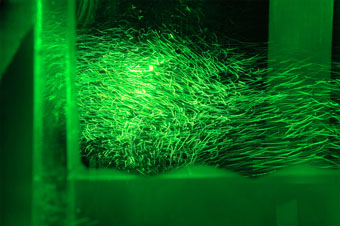
\includegraphics[width=0.47\textwidth]{stroemung3.PNG}
  \caption{Bildunterschrift}
  \label{fig:bild4}
\end{figure}
